% Source: graduate-coursework/Prior_Semesters/Fa25/EMCH501/HW3/HW3.tex
% Description: Visual representation of the initial temperature distribution (parabolic profile).

\documentclass[border=4pt]{standalone}
\usepackage{amsmath}
\usepackage{amssymb}
\usepackage{graphicx}
\usepackage{pgfplots}
\usepackage{tikz}
\usepackage{xcolor}
\pgfplotsset{compat=1.18}
\usetikzlibrary{shapes.geometric, arrows.meta, positioning, decorations.pathmorphing, patterns}

\definecolor{USC_Garnet}{HTML}{73000A}
\definecolor{USC_Sandstorm}{HTML}{FFF2E3}
\definecolor{USC_Black90}{HTML}{565656}
\definecolor{USC_Black10}{HTML}{ECECEC}
\definecolor{USC_Honeycomb}{HTML}{65780B}

\begin{document}
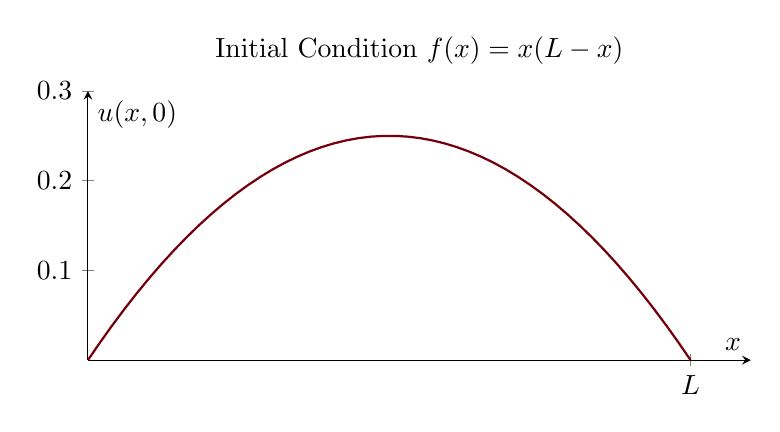
\begin{tikzpicture}[scale=1.0]
    \begin{axis}[
        axis lines=middle,
        xlabel=$x$, ylabel={$u(x,0)$},
        xmin=0, xmax=1.1,
        ymin=0, ymax=0.3,
        width=10cm, height=5cm,
        xtick={0, 1}, xticklabels={0, $L$},
        title={Initial Condition $f(x) = x(L-x)$}
    ]
    % Plotting x(1-x) as a normalized representation
    \addplot[thick, color=USC_Garnet, domain=0:1, samples=50] {x*(1-x)};
    \end{axis}
\end{tikzpicture}
\end{document}
